\documentclass[12pt,a4paper]{article}
\usepackage[utf8]{inputenc}
\usepackage[german]{babel}
\usepackage[T1]{fontenc}
\usepackage{amsmath}
\usepackage{amsfonts}
\usepackage{amssymb}
\usepackage{graphicx}
\usepackage[left=2cm,right=2cm,top=2cm,bottom=2cm]{geometry}
\author{Tim}

\begin{document}
\newpage
\tableofcontents
\newpage

\section{Versuchsbeschreibung}
Ziel des Versuches ist die Vermessung der Dampfdruckkurve und die Bestimmung der Verdampfungsenthalpie von Wasser.\\

Der Sättigungsdampfdruck wird quantitativ durch die Clausius-Clapeyron-Gleichung beim Phasenübergang flüssig-gasförmig beschrieben.

\begin{equation}
	\frac{dp}{dT}=\frac{\nu \Lambda}{T(V_{gas}-				V_{flüssig})}
\end{equation}

Da $V_gas >> V_flüssig$ folgt unter der Annahme das sich die Verdampfungsenthalpie $\Lambda$ innerhalb von kleinen Temperaturbereichen nicht ändert mittels Integration den für diesen Versuch entscheidenden Zusammenhang:

\begin{equation}
	\ln{(p/p_0)}=-\frac{\Lambda}{R} (\frac{1}{T}-			\frac{1}{T_0})
\end{equation}

Mit diesem Zusammenhang kann die Verdampfungsenthalpie $\Lambda$ für verschiedene Temperaturen bestimmt werden indem die Geradenanpassung um diese Punkte und innerhalb kleiner Temperaturänderungen stattfindet.

\section{Aufbau und Durchführung}
\begin{figure}
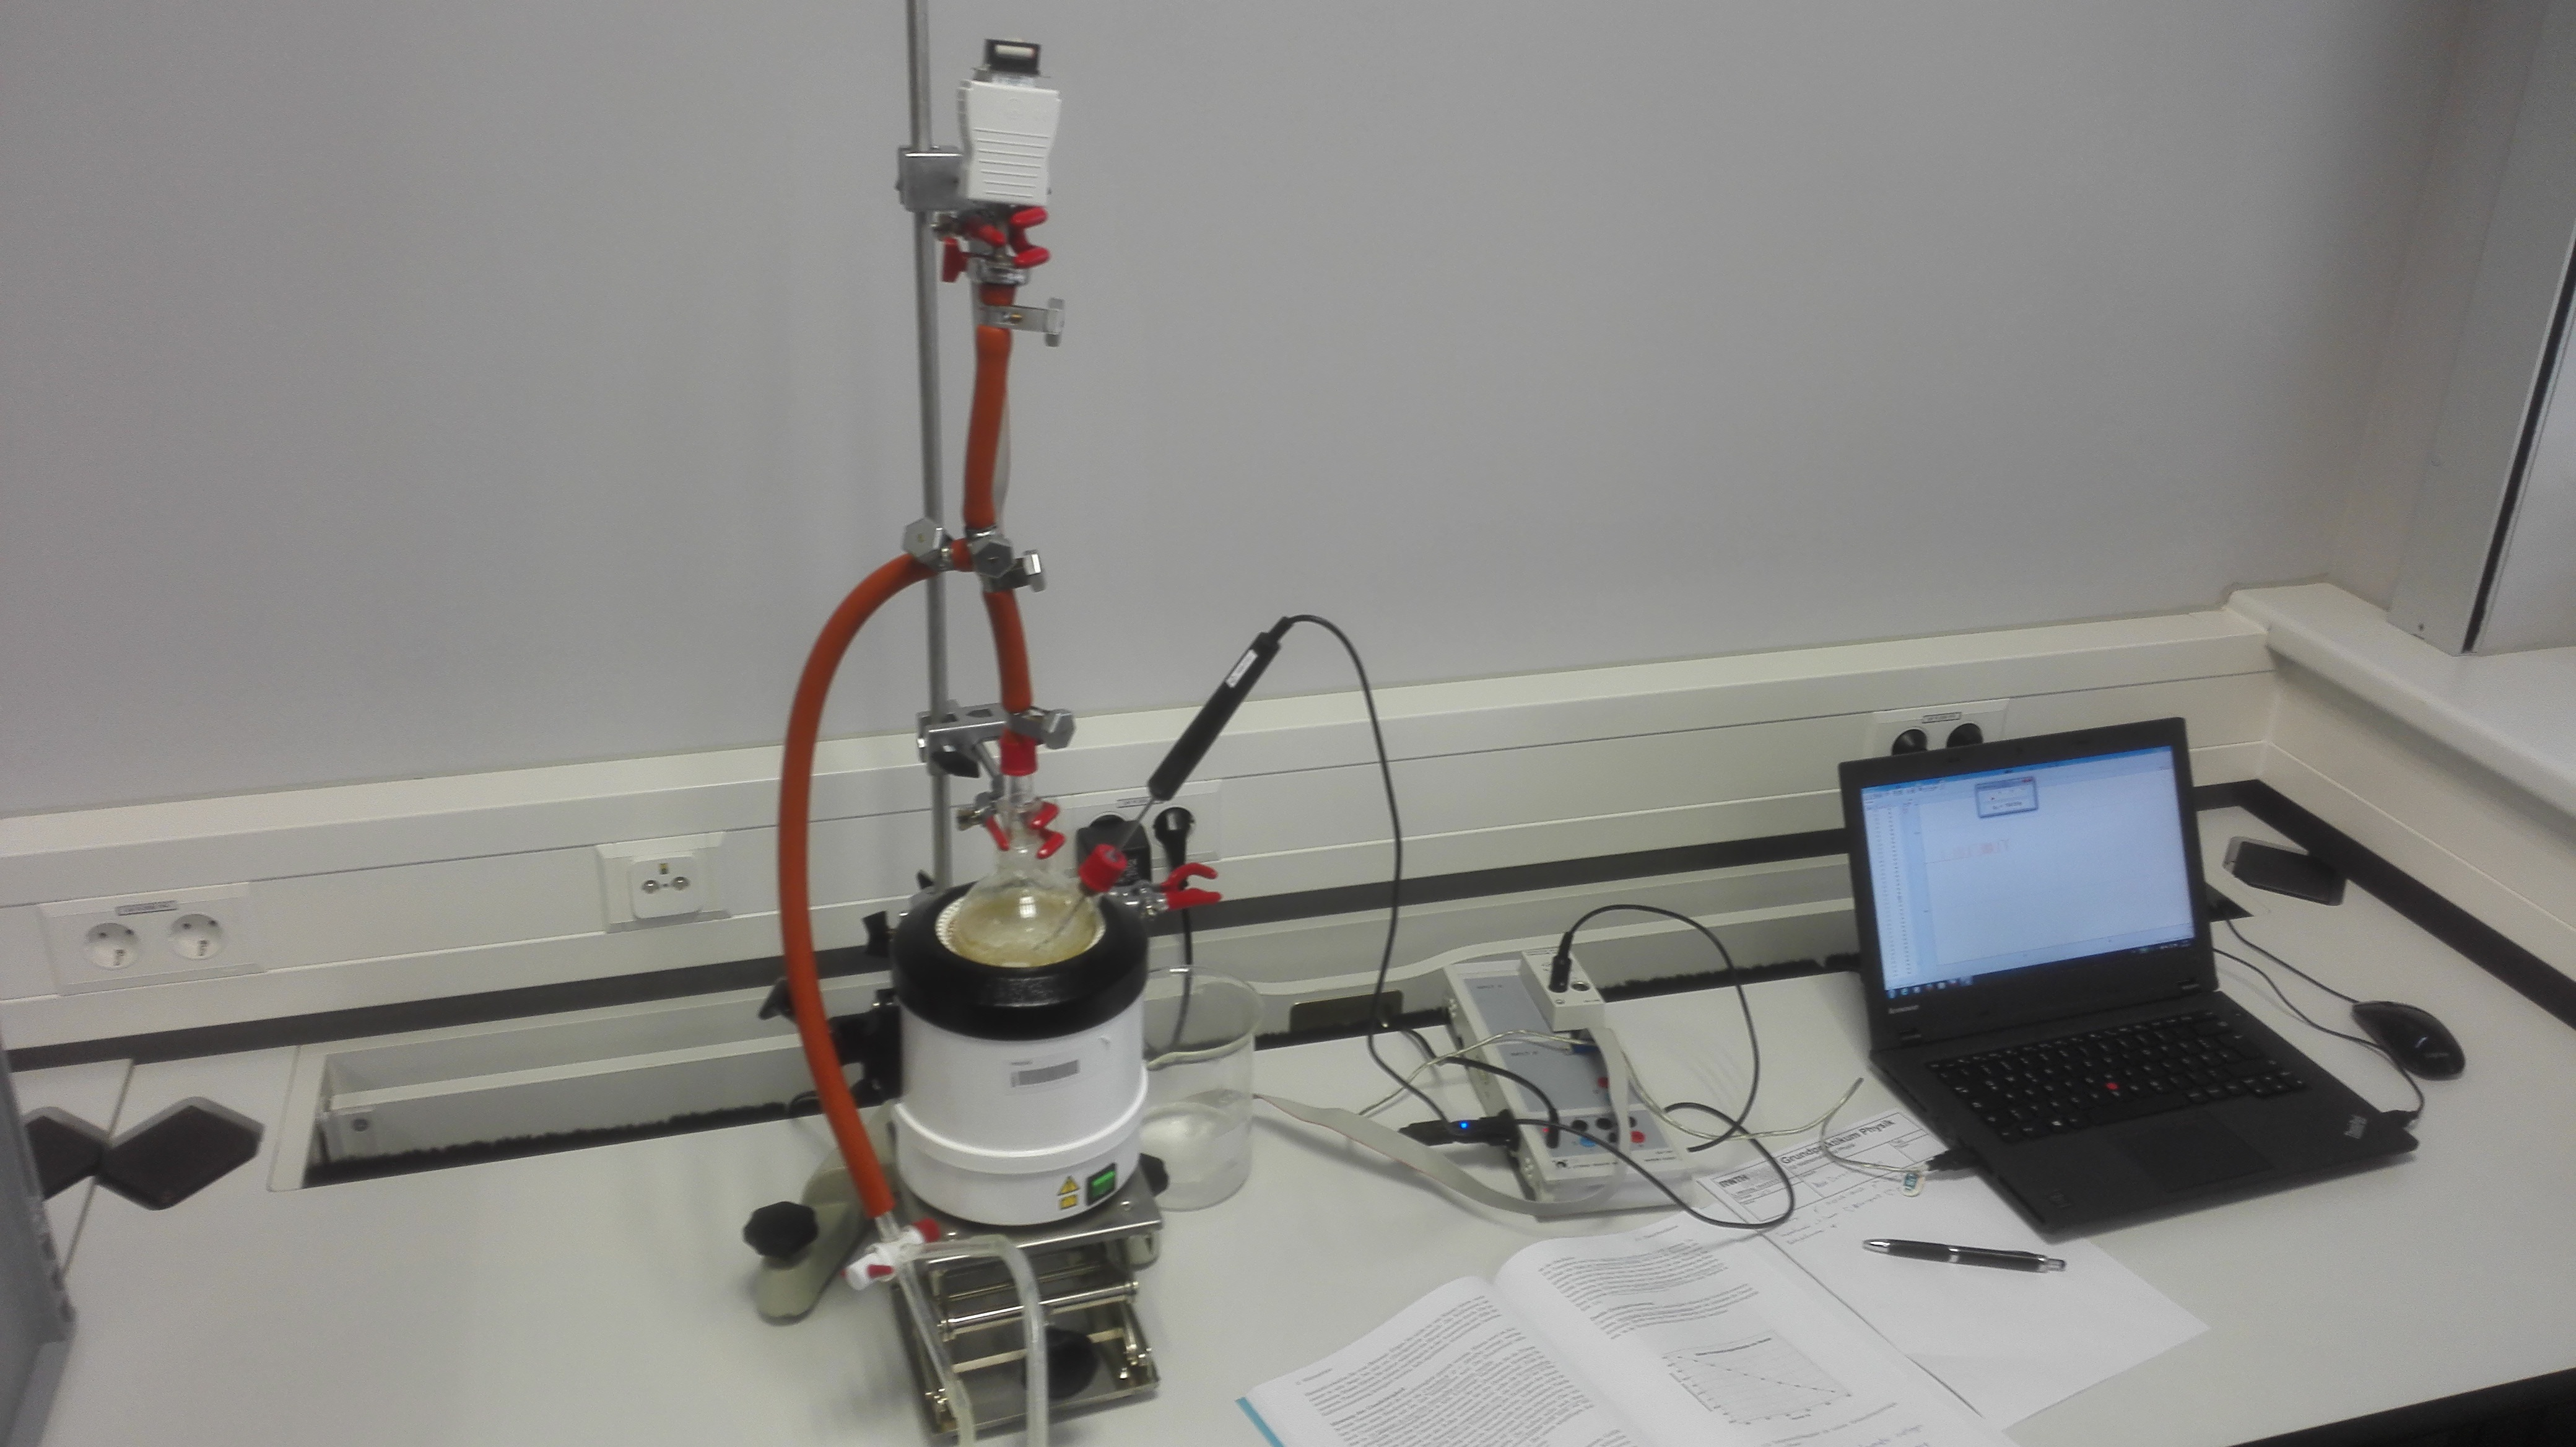
\includegraphics[width=\linewidth]{Bilder/AufbauB}
\caption[AufbauB]{Aufbau Versuch B}
\label{fig:AufbauB}
\end{figure}

Das Thermometer wird mit der Thermobox an das CASSY angeschlossen. Als Messbereich wird $-20C-120C$ gewählt. Es werden die Momentanwerte im Abstand von $1s$ aufgezeichnet.\\
Der Druckmesser ist direkt mit dem CASSY verbunden. Der Messbereich wird zu $0hPa-1500hPa$ gewählt. Auch hier wird jede Sekunde der Momentanwert gemessen.\\

Der Glaskolben wird etwa zur Hälfte mit Wasser gefüllt und über die entsprechenden Anschlüsse mit Temperaturfühler und Drucksensor verbunden. Sowohl der Kolben als auch die Messinstrumente werden am Stativ befestigt. Der Heizpilz wird auf dem ausgefahrenen Laborheber so unter den Kolben montiert, so dass er schnell entfernt werden kann. Eine Handpumpe wird über den Dreiwegehahn mit dem Kolben verbunden.\\

Die Rauschmessung der Sensoren wird zusammen mit der Kalibrierung des Temperaturfühlers durchgeführt. Dazu werden $300$ Messwerte aufgezeichnet.\\
Zur Überprüfung der Gasdichtigkeit wird mit der Handpumpe bei verschlossenem Auslass der Druck im Glaskolben auf weniger als $200hPa$ gesenkt und der weitere zeitliche Verlauf des Drucks gemessen.\\

Im Hauptversuch wird bei geöffnetem Auslass das Wasser im Glaskolben bis zum Sieden erhitzt. Hat man sich davon überzeugt das der Kolben keine Luft mehr enthält wird der Auslass geschlossen und der Heizpilz entfernt. Während des Abkühlens wird dann die Dampfdruckkurve aufgezeichnet bis das Wasser im Kolben aufhört zu sieden.\\
Am Ende des Messvorgangs lässt man das Wasser weiter abkühlen und führt gegebenenfalls eine zweite Dichtigkeitsmessung durch. 

\section{Versuchsauswertung}






\end{document}